\section{Protocolo de Comunicação}

\subsection{Problema de integração entre o AUVNetSim e o NM3}

Tendo em vista a proposta inicial que tinha como objetivo simular a comunicação de uma redes de sensores subaquáticos baseado no modelo de arquitetura de rede tridimensional com veículos autônomos subaquático ou AUV (do inglês, autonomous underwater vehicles)  \cite{akyildiz2005underwater} na simulação 3D do submarino BROV. Assim, conforme é apresentado na Figura \ref{fig:arquitetura-comunicacao-brov}, a finalidade era dispor aleatoriamente na área simulada, diversos modens acústicos que fariam a tráfego das informações entre o BROV, a boia e objeto a ser capturado (representado pela moeda) e um sensor SBL faria a transmissão dos dados de localização da moeda. 

\begin{figure}[h]
	\centering
	\caption[Arquitetura de Comunicação do BROV]{Arquitetura de Comunicação do BROV}
	\label{fig:arquitetura-comunicacao-brov}
	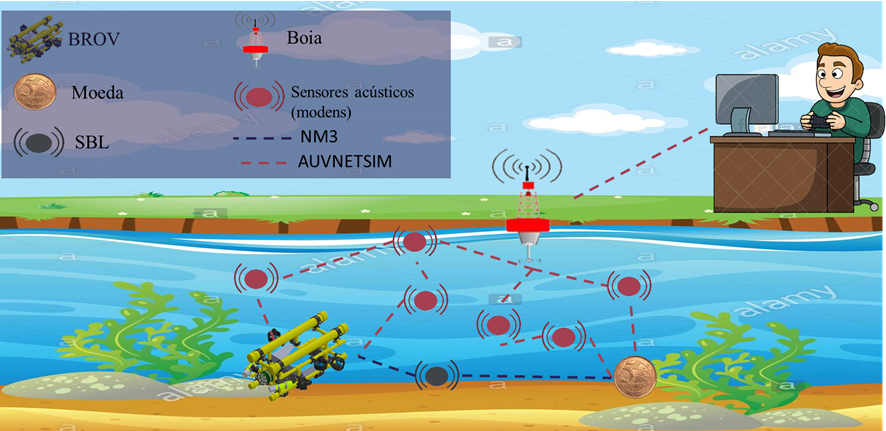
\includegraphics[width=0.8\linewidth]{images/arquitetura-comunicacao-brov}\\
	\footnotesize Fonte: Autores
\end{figure}


Desse modo, a comunicação seria simulada pelo simulador AUVNetSim pelo Josep Miquel Jornet Montana em um programa no MIT(do inglês, Massachusetts Institute of Technology) \cite{montana2008auvnetsim} e pela biblioteca python para os modens acústicos subaquáticos NM3 desenvolvida pela os laboratórios USMART( do inglês, Smart dust for large scale underwater wireless sensing) \cite{8248761}. Onde, a primeira tecnologia atuaria na simulação da comunicação entre os dispositivos em uma topologia de rede (em vermelho) com a arquitetura conforme proposto na Figura 5 e o NM3 para a comunicação do trilateração SBL (em preto) respectivamente, sendo ambas seriam integradas ao a simulação 3D, feitas pelo ROS e Igntion.

No entanto, diversos problemas e desafios foram encontrados o que inviabilizou a construção da simulação da rede subaquática, de modo geral, por causa do tempo de entrega do projeto ou por problemas com a integração com as tecnologias para simulação tridimensional. 

Em detalhes o AUVNetSim apresentou as seguintes dificuldades:

\begin{itemize}
	\item Para executar a ferramenta é necessário o uso do framework de ambiente para simulação de eventos discretos baseado no Python, chamado Simpy \cite{montana2008auvnetsim}, na versão 2.2. Esta versão em específico com executa com a linguagem de programação python 2, apesar de esforços para migrar grande parte do código fonte do AUVNetSim para o python 3, esta dependência não pode ser alterada devido ao tempo necessário.
	\item Com o objetivo de atender da melhor forma os requisitos de projeto voltados a simulação 3D, foi selecionado pela equipe de trabalho dentre outras ferramentas ROS 2 Rolling Ridley liberado em tecnologia funciona com o com o python 3 e que causa incompatibilidade no processo de integração com AUVNetSim, haja visto, que este executa com Python 2.
	\item Apesar da ciência da equipe de antemão que a ferramenta não emulava, mas apenas simulava a comunicação subaquática apresentado por fim todas as informações de colisão, delay, consumo de energia etc. A proposta inicial era modificar o código fonte da aplicação, já que a ela tem o código aberto (do inglês, open source), a fim de modificá-la para um emulador dentro simulação 3D, respeitando todos os processos normalmente feitos por um dispositivo em rede, como a transmissão de dados em camadas de protocolos de comunicação, só que, neste contexto, preparados para o ambiente subaquático. No entanto, a tentativa foi frustrada pela dificuldade na modificação do código conforme já mencionado.
\end{itemize}

O NM3 possui um protocolo de comunicação específicos em diversas camadas abstração (  camada física e MAC por exemplo) que tratam uma série de fatores que um dispositivo em rede no ambiente subaquático possui. Contudo, com intuito de se ter uma simulação mais próxima do mundo real, para usar esta biblioteca é necessário trabalhar no desenvolvimento dos cálculos relacionados a propagação som para a transmissão de dados, já que eles são feitos de forma muito simplificada, pois, não assumem perdas dados relacionadas a velocidade, obstruções, caminhos múltiplos ou ruído. Simplesmente, calcula o tempo de chegada do dado com base em uma velocidade nominal do som (1500 m / s) e a distância em linha reta entre o nó transmissor e o nó receptor. 

Todavia, a biblioteca permite alteração desses fatores relacionados aos cálculos de propagação de forma objetiva e simples, mas seu emprego foi inviabilizado por:

\begin{itemize}
	\item Ser necessário simular os modens na simulação 3D, já que programa foi desenvolvido para rodar no hardware produzido para ele.
	\item Complexidade associadas a configuração da rede, já que a comunicação é feita por meio da conexão via porta serial.
\end{itemize}




\subsection{Nova abordagem para simulação da comunicação}

Conforme citado no subtópico acima, a simulação da comunicação por meio de uma rede de sensores subaquáticos foi abortada pelos motivos mencionados. Desse modo, com a intenção de se ter uma simulação para fidedigna do ambiente físico, foi pensado em cálculo básico para se obter o delay\footnote{Delay é o tempo de processamento ou velocidade dos equipamentos e softwares de captura e recebimento de dados.}  da transmissão de dados entre os dispositivos (BROV, moeda e boia) no meio subaquático, descritos no próximo subtópico.

Sendo assim, como pode ser visto no esboço apresentado na Figura \ref{fig:aplicacao-delay} foi elaborado uma proposta que a estrutura de conexão ou ponte de conexão entre a simulação 3D e ROS, interceptaria o envio e recebimentos de dados (comandos) dos sensores dos dispositivos simulados, assim como as suas respectivas poses (ou posições na simulação).

\begin{figure}[h]
	\centering
	\caption[Esboço de esquema para aplicação de delay]{Esboço de esquema para aplicação de delay}
	\label{fig:aplicacao-delay}
	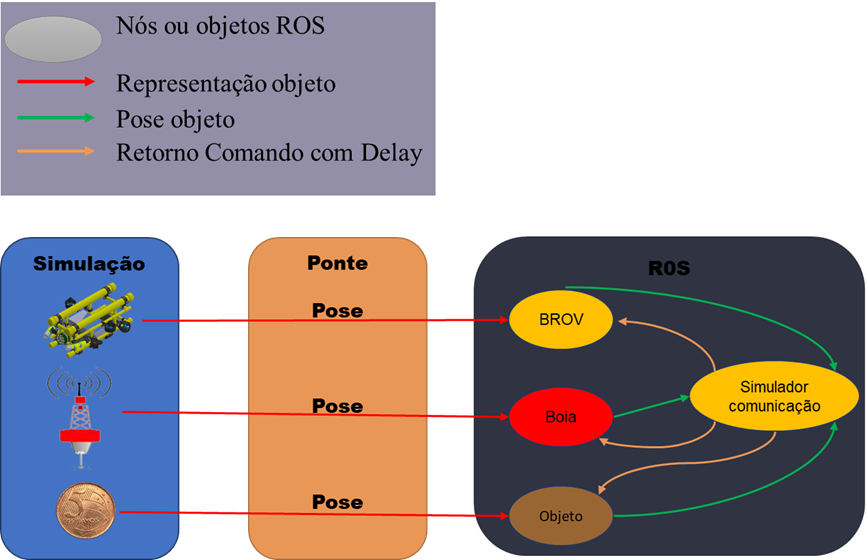
\includegraphics[width=0.8\linewidth]{images/aplicacao-delay}\\
	\footnotesize Fonte: Autores
\end{figure}


De modo, que dentro ambiente ROS um node ou serviço receberá estes dados, calculará, aplicará e retornará o comando com o tempo de delay de acordo com distância entre eles no ambiente simulado. Por exemplo. Quando o operador dar comando ao por meio do Joystick,  a boia que recebe o comando da estação em terra, deverá enviar o comando para o AUV programado previamente no ROS, neste processo é coletados a posição dos objetos (boia e BROV), aplicado o tempo de delay antes de animação de movimento do BROV chegar na simulação.

É importante mencionar que a implementação desta abordagem só é útil no contexto de simulação, sendo desnecessária no ambiente real.

\subsection{Equação de \textit{delay}}

Tempo de delay é representado pela razão entre a distância pela velocidade do som na água, sendo dada pela equação \ref{eq:delay} a seguir.

\begin{equation}
	delay = \dfrac{dist\hat{a}ncia_{AB}}{velocidade\;do\;som\;na\;\acute{a}gua}
	\label{eq:delay}
\end{equation}

A $dist\hat{a}ncia_{AB}$ entre dois objetos $A = (x_a,y_a,z_a)$ e o objeto $B = (x_b,y_b,z_b)$ na simulação dada por meio de suas coordenadas $(X, Y e Z)$ é calculada por meio da equação \ref{eq:distancia}. 

\begin{equation}
	dist\hat{a}ncia_{AB} = \sqrt{(X_B + X_A)^2 + (Y_B + Y_A)^2 + (Z_B + Z_A)^2}
	\label{eq:distancia}
\end{equation}

A velocidade do som pode ser calculada em função da temperatura da água do mar, salinidade e pressão, profundidade ou latitude. Para este fim, foi encontrado no estado arte as equações mackenzie, coppens e UNESCO, todas elas são descritas e referenciadas na página “Technical Guides - Speed of sound in sea water” disponível neste \href{http://resource.npl.co.uk/acoustics/techguides/soundseawater/index.html}{link} (veja na Figura \ref{fig:npl} logo abaixo)  pelo National Physical Laboratory, que ainda disponibiliza uma calculadora para calcular a velocidade do som na água do mar.

\begin{figure}[h]
	\centering
	\caption[Imagens do print do site Technical Guides - Speed of sound in sea water]{Imagens do print do site Technical Guides - Speed of sound in sea water}
	\label{fig:npl}
	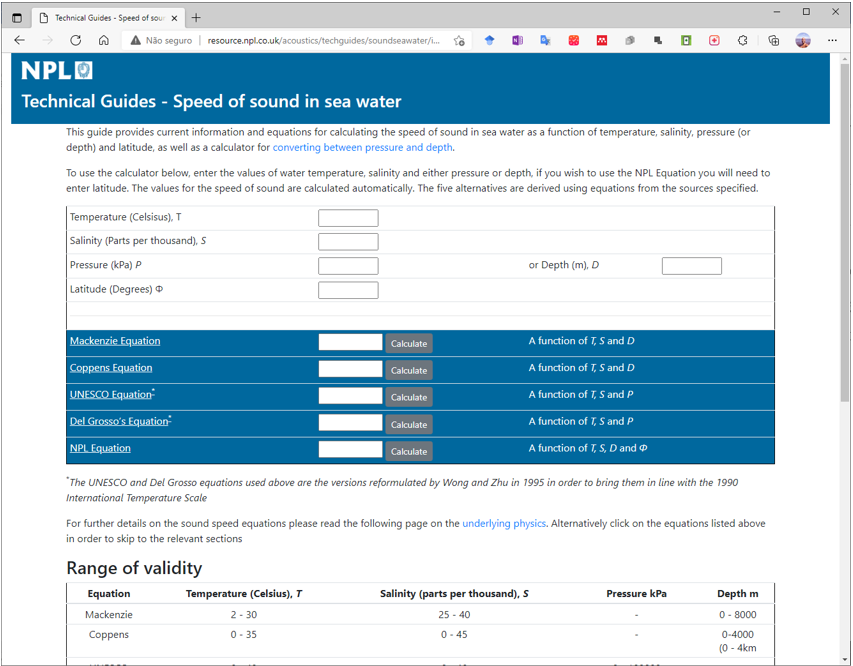
\includegraphics[width=0.8\linewidth]{images/npl}\\
	\footnotesize Fonte: \cite{techinical}
\end{figure}


A Equação \ref{eq:mackenzie} criada por Mackenzie em 1981 calcula a velocidade do som na água do mar em função de T (temperatura em graus Celsius), S (salinidade partes por mil) e D (profundidade em metros), sendo que sua validade está nas faixas de temperatura de 2 a 30 °C, salinidade de 25 a 40 partes por mil e profundidade de 0 a 8000 m \cite{simpy}.

\begin{equation}
\begin{aligned}
	c(D,S,T) = & 1448,96 + 4.591T - 5.304 \times 10^{-2}T^2 + 2.374 \times 10^{-4}T^3 + 1.340 (S-35)\\ & + 1.630 \times 10^{-2}D + 1.675 \times 10^{-7}D^2 - 1.205 \times 10^{-2}T(S-35)\\& - 7.139 \times 10^{-13}TD^3
\end{aligned}
\label{eq:mackenzie}
\end{equation}

A Equação \ref{eq:coppens} criada por Coppens em 1981 calcula a velocidade do som na agua do mar em função de t = T/10 (onde T = temperatura em graus Celsius), S(salinidade partes por mil) e D (profundidade em quilômetros), sendo que sua validade estão nas faixas de temperatura de 0 a 35 °C, salinidade de 0 a 45 partes por mil, profundidade de 0 a 4000 m \cite{simpy}.

\begin{equation}
\begin{aligned}
	c(D,S,T) = & c(0,S,t) + (16,23 + 0,253t)D + (0,213 - 0,1t)D^2\\ & + [0,016 + 0,0002(S-35)](S-35)tD\\	
	c(0,S,t) = & 1449,05 + 45,7t - 5.21t^2 + 0,23t^3\\ & +(1.333 - 0.126t + 0.009t^2)(S-35)
\end{aligned}
\label{eq:coppens}
\end{equation}

A Equação UNESCO em \ref{eq:unesco} criada por Chen and Millero em 1981 e recalculada 1995pela última vez. Calcula a velocidade do som na agua do mar em função de T (temperatura em graus Celsius), S(salinidade partes por mil) e P (pressão em bar), sendo que sua validade estão nas faixas de temperatura de 0 a 40 °C, salinidade de 0 a 40 partes por mil, pressão de 0 a 1000 bar \cite{simpy}.

\begin{equation}
	\begin{aligned}
		c(S,T,P) = & Cw(T,P) + A(T,P)S + B(T,P)S^{\frac{3}{2}} + D(T,P)S^2\\	
		Cw(T,P) = & (C_{00} + C_{01}T + C_{02}T^2 + C_{03}T^3 + C_{04}T^4 + C_{05}T^5)+\\
		& (C_{10} + C_{11}T + C_{12}T^2 + C_{13}T^3 + C_{14}T^4)P+\\
		& (C_{20} + C_{21}T + C_{22}T^2 + C_{23}T^3 + C_{24}T^4)P^2+\\
		& (C_{30} + C_{31}T + C_{32}T^2)P^3\\
		A(T,P) = & (A_{00} + A_{01}T + A_{02}T^2 + A_{03}T^3 + A_{04}T^4)+\\
		& (A_{10} + A_{11}T + A_{12}T^2 + A_{13}T^3 + A_{14}T^4)P+\\
		& (A_{20} + A_{21}T + A_{22}T^2 + A_{23}T^3 + A_{24}T^4)P^2\\
		& (A_{30} + A_{31}T + A_{32}T^2)P^3\\
		B(T,P) = & B_{00} + B_{01}T + (B_{10} + B_{11}T)P\\
		D(T,P) = & D_{00} + D_{10}P
	\end{aligned}
	\label{eq:unesco}
\end{equation}


\subsection{Considerações finais sobre a comunicação}

Com o objetivo de disponibilizar e aumentar os parâmetros para casos de testes e análises no futuro, todas as três equações citadas foram implementas e estão disponíveis no código fontes neste \href{https://github.com/maxsilva24/comunicao_subaquatica_brov}{link}. Contudo, vale destacar que a equação 5 (UNESCO) está com um erro na 8ª casa decimal, a validação foi feita em comparação com os resultados apresentados pela calculadora na página\textit{ Technical Guides - Speed of sound in sea water}. Além disso, ainda existe mais uma equação para calcular a velocidade do som na água do mar, a NPL desenvolvida pelos autores Leroy, Robinson e Goldsmith em 2008, que não foi implementada no código disponibilizado.

Por fim, as modificações no código fontes do AUVNetSim, bem como a descrição do passo a passo utilizados para executá-lo conforme print apresentado na Figura \ref{fig:print-auvnetsim}, também disponíveis no repositório citado.

\begin{figure}[h]
	\centering
	\caption[Print da dela com a execução do AUVNetSim]{Print da dela com a execução do AUVNetSim}
	\label{fig:print-auvnetsim}
	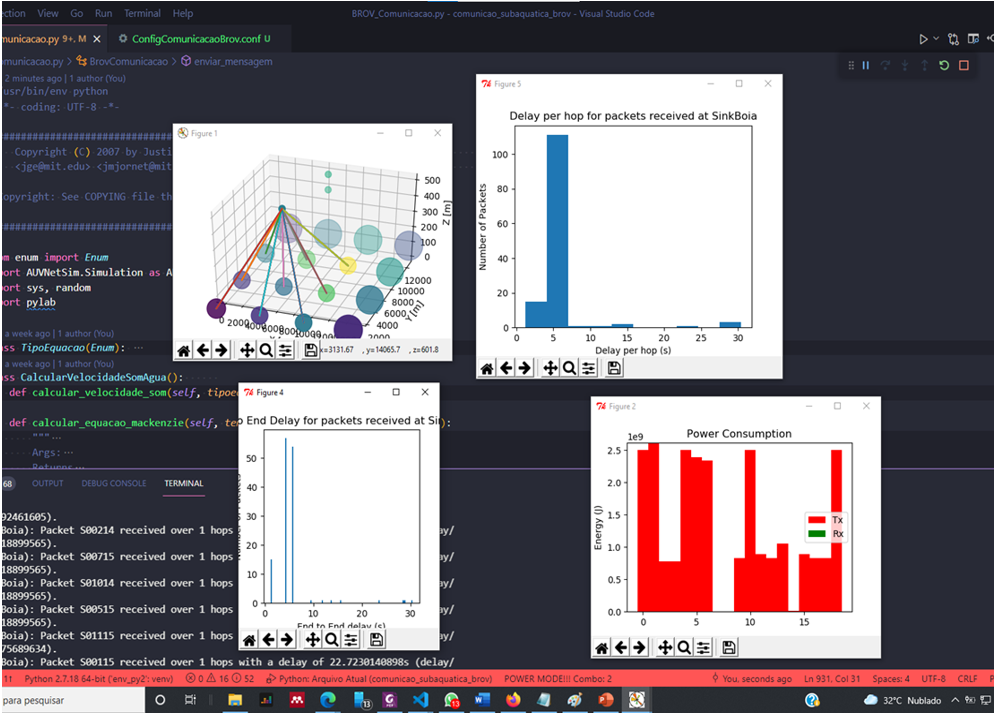
\includegraphics[width=0.8\linewidth]{images/print-auvnetsim}\\
	\footnotesize Fonte: Autores
\end{figure}
